\documentclass[11pt,twocolumn]{article}
\IfFileExists{acl.sty}{%
  \usepackage[final]{acl}
}{%
  \usepackage[margin=0.75in]{geometry}
  \setlength{\columnsep}{0.25in}
}
\usepackage{latexsym}
\usepackage{amsmath}
\usepackage{booktabs}
\usepackage{graphicx}
\usepackage{xcolor}
\usepackage{url}
\usepackage{tikz}
\usetikzlibrary{positioning, arrows.meta, shapes.geometric, fit, calc, backgrounds}

\makeatletter
\renewcommand{\verbatim@font}{\normalfont\ttfamily\footnotesize}
\makeatother
\setlength{\emergencystretch}{6em}

\definecolor{ink}{RGB}{24,31,42}
\definecolor{muted}{RGB}{92,105,122}
\definecolor{rline}{RGB}{205,213,224}
\definecolor{red}{RGB}{176,42,55}
\definecolor{gold}{RGB}{220,158,28}
\definecolor{teal}{RGB}{15,118,110}
\definecolor{blue}{RGB}{37,99,235}
\definecolor{green}{RGB}{22,163,74}
\definecolor{orange}{RGB}{234,88,12}
\definecolor{purple}{RGB}{124,58,237}
\definecolor{soft}{RGB}{246,248,251}
\definecolor{warmsoft}{RGB}{255,246,230}
\definecolor{coolsoft}{RGB}{232,246,240}

\tikzset{
  block/.style    ={rectangle, rounded corners=2pt, draw=rline, fill=soft,
                    inner sep=4pt, minimum height=22pt, font=\small, align=center},
  hostblock/.style={block, fill=warmsoft, draw=orange},
  encblock/.style ={block, fill=coolsoft, draw=green},
  awsblock/.style ={block, fill=soft, draw=rline},
  arr/.style      ={->, >={Stealth[length=2.2mm]}, thick, color=ink},
  thinarr/.style  ={->, >={Stealth[length=1.8mm]}, semithick, color=muted},
  zonelabel/.style={font=\scriptsize\bfseries, color=muted, anchor=north west},
}

\title{Plywood Analyzer: A Program-Analysis Evidence Workbench for AI-Generated C++}
\author{Sukeerth Kolakaluri, Likhitha Nakka, Rupa Kowshika Achanta}

\begin{document}
\maketitle

\begin{abstract}
Plywood Analyzer studies an AI-generated C++ plywood cut calculator with
static and dynamic program-analysis techniques. The pipeline stores program
structure in Neo4j, stores execution evidence in SQLite, and exposes the
evidence through a Flask query interface. The current target,
\path{src/plywood_calc.cpp}, is 246 lines and reaches 98.7\% gcov
line-block coverage, 0 scan-build defects, 29/29 differential-test matches,
and 24 cross-call dependency edges for Q2 dependency-path checks. The research
result is the cross-store join: one query combines static reachability from
Neo4j with dynamic coverage from SQLite and points to the only reachable
uncovered handler.
\end{abstract}

\section{Problem and Project Scope}

The assignment starts from a plain-language code-generation request, not from a
formal specification:

\begin{quote}
Let us build a small app that is a calculator. Input the dimensions
of a piece of plywood, and then it should calculate the resulting
size. The users are just normal people. The users are asked for the
plywood size, we give input like L * W. Then we ask the user what
smaller pieces they want, which is l * w. After that, we automatically
calculate how much smaller pieces are able to be cut, then we give a
visualization on how the cuts are made. For the code to realize it,
I prefer C/C++.
\end{quote}

\paragraph{Target.}
The program under analysis is \path{src/plywood_calc.cpp}, a 246-line
AI-generated C++ file (\cite{codex,pearce,lostatc,vaithilingam}). It reads board and cut dimensions, rejects nonpositive
or over-limit dimensions, computes the best normal or rotated cut count, prints
waste, and renders an ASCII layout. The workbench treats that file as the whole
program. It does not claim whole-repository C++ analysis.

\paragraph{Questions.}
The evaluated core has three deterministic questions. Q1 asks for caller and
callee relationships for a named function. Q2 asks whether two variables have a
dependency path inside a selected function. Q3 asks which functions reachable
from \texttt{main} contain uncovered gcov line-blocks. The repository also
contains two extension paths, Q4 and natural-language querying, that are
implemented in the CLI and Flask infrastructure but treated as future
evaluation work rather than as the main three-question claim.

\section{Design Document (10\%)}

\subsection{Static Analysis Component}

\paragraph{IR and graphs.}
\path{scripts/run_pipeline.sh} emits LLVM IR \cite{llvm} with
\texttt{clang++ -S -emit-llvm -g -O0}. The \texttt{-g} flag matters because
\path{analysis/dep_extractor.py} reads debug metadata rather than reporting
only SSA registers. \texttt{opt -dot-callgraph} then produces a call graph with
6 user functions and 6 user-level \texttt{CALLS} edges: \texttt{main} calls
\texttt{validate\_dimensions}, \texttt{get\_input}, \texttt{calculate\_cuts},
\texttt{print\_result}, and \texttt{render\_visualization};
\texttt{get\_input} also calls \texttt{validate\_dimensions}. The CFG lane uses
\texttt{opt -dot-cfg}. The live graph summary used by the interface reports 97
\texttt{BasicBlock} nodes and 56 \texttt{SUCCESSOR} edges.

\paragraph{Source-level dependencies.}
The dependency extractor walks \texttt{llvm.dbg.declare} records so Q2 can ask
about source-level dependence \cite{pdg} using names such as
\texttt{board.length} instead of \texttt{\%0}. It also resolves struct field
accesses from \texttt{getelementptr}. The Task 11 extension bridges call
boundaries so Q2 can follow dependencies across helper calls and value-passing
conventions \cite{andersen}. It handles pointer-typed arguments, such as
\texttt{get\_input(\&board, \&cut)}, and the packed-by-value ABI shape that LLVM
uses for small structs passed to \texttt{calculate\_cuts},
\texttt{print\_result}, and \texttt{render\_visualization}. In the current
\path{data/dependencies.json}, the extractor writes 117 dependency rows,
including 24 cross-call rows.

\paragraph{Clang Static Analyzer.}
The static-bug pass uses \texttt{scan-build-14} around \texttt{clang++-14}
\cite{coverity}.
The recorded output in \path{data/scan-build-output.txt} says ``No bugs
found.'' That result is useful but narrow: it is a path-sensitive C/C++ checker
run, not a proof that allocation sizes or integer products are safe under every
future edit. The implementation is a project-specific pass over
common compiler structures (see \cite{aho,nielson} for the underlying theory).

\subsection{Dynamic Testing Component}

\paragraph{Curated tests and oracle.}
The three files matching \path{tests/ai_generated_*.txt} expand to 29
CSV-style command-line tests in \path{data/test_results.json}. The first
version of the harness could have counted a test as passing when the process
returned 0. The current harness is stricter. \path{analysis/reference_calc.py}
implements the cut-count rule through differential testing \cite{mckeeman}
(in the lineage of property-based random testing, \cite{quickcheck}):
\[
\max\left(
\left\lfloor \frac{BL}{CL} \right\rfloor
\left\lfloor \frac{BW}{CW} \right\rfloor,\,
\left\lfloor \frac{BL}{CW} \right\rfloor
\left\lfloor \frac{BW}{CL} \right\rfloor
\right).
\]
Each binary run must match that value, with rejected inputs represented as
\texttt{None}. The current result is 29/29 matches.

\paragraph{Coverage.}
\path{analysis/coverage_collector.py} runs the tests against
\path{build/plywood_calc_cov}, invokes gcov \cite{gcov}, and writes line-block rows for
SQLite. The live database has 150 \texttt{coverage} rows. Effective coverage is
148/150 line-blocks, or 98.7\%. Every line-block in
\texttt{validate\_dimensions}, \texttt{calculate\_cuts}, \texttt{get\_input},
\texttt{print\_result}, and \texttt{main} is hit. The two misses are in
\texttt{render\_visualization}, lines 163--164, the \texttt{malloc} failure
handler.

\paragraph{Fuzzing.}
AFL++ \cite{afl,aflpp} runs from the same structured four-integer input shape. The recorded run
in \path{data/fuzz_stats.json} completed 166,707 executions in 58 seconds,
recorded 71 total paths, and reported 0 crashes and 0 hangs. The replay step in
\path{scripts/replay_afl_queue.sh} runs each of the 71 queue inputs through the
gcov binary and tags the resulting rows as \texttt{gcov\_afl\_replay}. On this
target, replay added 0 new line-blocks beyond the curated coverage. That is a
coverage-guided fuzzing finding \cite{aflfast} about this program and seed
shape, not a pipeline failure.

\subsection{Storage}

\paragraph{Neo4j.}
Neo4j \cite{neo4j} stores the static program graph. It has \texttt{Function},
\texttt{BasicBlock}, and \texttt{Variable} nodes, plus \texttt{CALLS},
\texttt{ENTRY\_BLOCK}, \texttt{SUCCESSOR}, and \texttt{DEPENDS\_ON} edges.
This store fits recursive graph questions. A call-chain search is one Cypher
pattern, \texttt{[:CALLS*0..10]}, and a Q2 data-dependency answer is a
\texttt{shortestPath} query over \texttt{DEPENDS\_ON}.

\paragraph{SQLite.}
SQLite stores dynamic evidence. The current \path{data/coverage.db} has
150 rows in \texttt{coverage}, 29 rows in \texttt{test\_cases}, and 1 row in
\texttt{fuzz\_stats}. SQL fits this evidence because the common operations are
grouping by function, taking \texttt{MAX(hit\_count)} across source tags, and
counting uncovered blocks.

\paragraph{Why two stores.}
Q3 needs both stores. Neo4j knows which functions are reachable from
\texttt{main}; SQLite knows which gcov line-blocks were not hit. Neither store,
alone, answers ``reachable and uncovered'' without copying the other store's
facts into it.

\subsection{Query Interface}

\paragraph{Q1: call graph.}
Q1 runs a parameterized Cypher lookup over \texttt{CALLS}. With
\texttt{func=main}, the canonical answer is that no user function calls
\texttt{main}, and \texttt{main} calls \texttt{calculate\_cuts},
\texttt{get\_input}, \texttt{print\_result}, \texttt{render\_visualization},
and \texttt{validate\_dimensions}. The same code path backs the CLI and Flask
views in \path{query_system/query_engine.py}.

\paragraph{Q2: dependency path.}
Q2 asks for a shortest dependency path between two variables, scoped by
function when the caller provides function names. For example, the live fallback
path for \texttt{vis\_height} to \texttt{grid} inside
\texttt{render\_visualization} has depth 1. That answer comes from the
\texttt{malloc(vis\_height * vis\_width * sizeof(char))} line.

\paragraph{Q3: reachability joined with coverage.}
Q3 first asks Neo4j for functions reachable from \texttt{main} with
\texttt{[:CALLS*0..10]}. It then asks SQLite for effective coverage with a CTE
that groups by block and takes \texttt{MAX(hit\_count)}. The canonical answer is
specific: \texttt{render\_visualization} has 2 uncovered line-blocks out of 59,
lines 163--164. The join keeps the result focused on code reachable from the
entry point. In the Flask interface, this answer is not only a table row: the
Q3 card links to the source panel, where
\path{/api/source/highlights?kind=uncovered} marks the exact reachable-but-untested
handler lines.

\paragraph{Implemented extensions.}
The codebase already contains two research extensions beyond the evaluated core.
Q4 composes the same evidence stores to ask which variables written by
\texttt{get\_input} can flow, through dependency edges, into functions that Q3
marks as reachable and uncovered. In the current snapshot, it reports
\texttt{render\_visualization} as the uncovered sink scope and returns an
example path from the input-side \texttt{board} value to the visualization
argument. This is best described as a taint-reachability prototype: it reuses
the cross-call dependency graph, but it does not yet model sanitizers,
control-dependence predicates, or aliasing strongly enough to claim a full
taint analysis.

The Flask route \path{/api/query} and the CLI \texttt{--ask} path implement a
natural-language query front end. The translator maps a user question to either
Cypher over Neo4j or SQL over SQLite, then returns the generated query and
result. This is an interface extension over the same storage design rather than
a separate analysis. The research direction is to constrain the generated
queries to a verified subset, evaluate semantic accuracy against a fixed query
suite, and attach provenance so a natural-language answer can still be traced
back to the graph or coverage rows that support it.

\begin{figure*}[t]
\centering
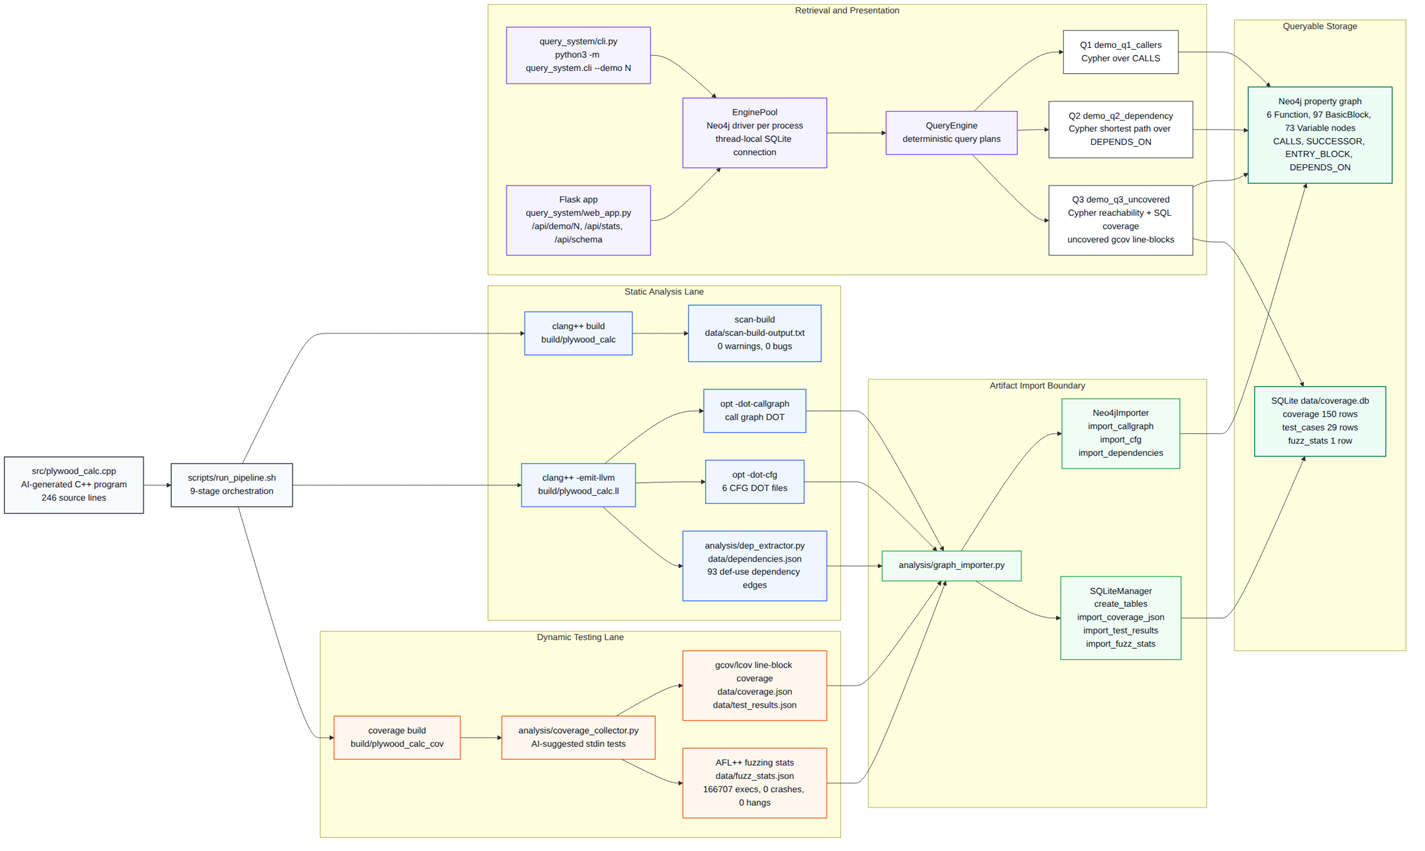
\includegraphics[width=0.95\linewidth]{image.png}
\caption{Pipeline from source to LLVM IR, static and dynamic analysis lanes,
Neo4j and SQLite stores, and the Flask query interface.}
\label{fig:pipeline}
\end{figure*}

\section{Research Report on AI-Generated Code}

\subsection{Can AI successfully generate the designed code?}

On this prompt, yes at the level a user would first notice \cite{codex}. The program
compiles, accepts the intended four dimensions, rejects nonpositive values, and
prints plausible counts and layouts. The stronger answer depends on the oracle.
If passing meant only ``the process returned 0,'' all positive curated tests
would pass. The differential oracle in \path{analysis/reference_calc.py} is a
better check because it recomputes the expected count with the normal and
rotated formulas. Under that oracle, the binary still matches 29/29 curated
cases. That is a real success for this prompt, not just a lucky run, and it
matches the gap between developer expectation and experience reported for code
generation tools \cite{vaithilingam}.

The generated code also got several small decisions right. In
\texttt{calculate\_cuts}, it compares the normal and rotated cut counts and
keeps the row and column counts for the chosen orientation. In
\texttt{render\_visualization}, it returns early when \texttt{malloc} fails and
frees \texttt{grid} on the normal path. The current file also has a
\texttt{MAX\_BOARD\_DIM} check and checks every \texttt{scanf} return value, so
I do not count those as missing in this snapshot. The missing design work is
narrower: allocation-size arithmetic is still written as an \texttt{int}
product, the program has no sanitizer-backed contract, AFL has no input
dictionary, and there is no test that forces the allocation-failure handler.

\subsection{Do static analysis and testing help understand AI-generated code? In what way?}

They help most when they turn a code-reading task into a small evidence query.
The call graph gives a fast map of the program before reading the source
linearly. Q1 with \texttt{func=main} shows that \texttt{main} dispatches to
input handling, validation, cut calculation, result printing, and layout
rendering. For a reviewer opening \path{src/plywood_calc.cpp} cold, that answer
is a better first screen than scrolling.

Coverage gives a second kind of orientation. The CFG and gcov evidence show
that the curated tests exercise every line-block in
\texttt{validate\_dimensions}, \texttt{calculate\_cuts}, \texttt{get\_input},
\texttt{print\_result}, and \texttt{main}. Only
\texttt{render\_visualization} has misses, and Q3 names the exact lines:
163--164, the allocation-failure branch. That keeps the review from treating
``98.7\%'' as a vague comfort number. It names the gap and the owning function.
The web interface then turns that fact into an inspection workflow by opening
the source view with the missed reachable lines highlighted.

The differential oracle is the clearest correctness check. The reference
implementation is short enough to inspect by hand, and it encodes the core
semantic rule rather than a transcript of expected output. If the binary and
reference disagree, the failure is tied to a formula, not to formatting.

Q3 was the most useful combined query. It does not merely list uncovered code.
It asks whether the uncovered code is reachable from \texttt{main}. That
separates dead or out-of-scope coverage gaps from reachable handlers that tests
miss. For this file, Q3 says the only reachable miss is the
\texttt{malloc}-failure branch in \texttt{render\_visualization}.

\subsection{What types of bugs or weaknesses did you find?}

The current evidence does not show a correctness or memory bug in the
unmodified target. The differential oracle passes 29/29 cases, so every
archived test agrees with the reference cut-count calculation. The
scan-build run reports 0 defects. AFL ran for 58 seconds, completed 166,707
executions, explored 71 paths, and found no crashes or hangs. The only
uncovered region reported by the workbench is the \texttt{malloc}-failure
handler in \texttt{render\_visualization}, lines 163--164. That is honest
error handling, not a bug.

The allocation call on line 161 still deserves a note \cite{pearce,lostatc}: it
computes \texttt{vis\_height * vis\_width}, an input-derived size
\cite{newsome}, with \texttt{int} arithmetic before
\texttt{malloc} receives a byte count, and there is no \texttt{size\_t} guard
around that product. In this version, the visualization caps keep the product
small, and AFL with structured four-integer seeds did not reach the
\texttt{INT\_MAX} regime within this budget. We document the expression as a
static observation from manual inspection of the source, motivated by Q3
pointing at \texttt{render\_visualization}, not as a triggered failure.

\subsection{Was the finding from manual inspection or program analysis?}

The reachability finding came from program analysis \cite{coverity}: Q3 combines
Neo4j call reachability with SQLite coverage. The query identifies
\texttt{render\_visualization} as
reachable from \texttt{main} and as the only function with uncovered gcov
blocks, then points to lines 163--164. The malloc-size-arithmetic observation
came from manual reading of \texttt{render\_visualization} after Q3 narrowed
the review target. I inspected the allocation on line 161 and noted that the
multiplication is performed in \texttt{int} before conversion to
\texttt{malloc}'s size argument. Both steps are reproducible from the
workbench: run Q3 to list the reachable uncovered handler, then open the cited
source range and inspect the allocation/handler pair. The workbench supplies
the target and evidence; the size-arithmetic note is the human interpretation
of that target.

\section{Self Evaluation and Limits}

Plywood Analyzer is intentionally narrow. It analyzes one 246-line C++ file,
not a multi-file build with headers, templates, and libraries. The dependency
extractor is a source-level def-use approximation; it does not implement alias
analysis \cite{andersen}, control dependence, symbolic bounds, or sanitizer
semantics. AFL ran
for 58 seconds on structured four-integer seeds, so its 0-crash result should
not be read as deep fuzz assurance. These limits are visible in the query
answers, which is better than hiding them behind a larger dashboard.
Future work would add symbolic execution on \texttt{calculate\_cuts} \cite{klee}
and promote the implemented extensions into evaluated contributions. For Q4,
that means validating the taint-reachability result against hand-labeled data
and extending the dependency model with alias, control, and sanitizer facts. For
natural-language querying, it means replacing ad hoc prompt success with a
benchmark of supported questions, a query-safety policy, and provenance links
from each answer back to the exact Cypher or SQL evidence.

\section{Conclusion}

The workbench answers concrete questions about AI-generated C++ by tying each
answer to evidence. LLVM and the dependency extractor describe structure;
gcov, differential tests, scan-build, and AFL describe behavior; Neo4j and
SQLite keep each kind of evidence in the store that fits it. The result that
matters is the join across those pillars. Q3 finds the only reachable uncovered
handler and demonstrates the workbench contribution. The static-analysis
contribution is the cross-call dependency extraction that lets Q2 follow value
relationships across function boundaries. The existing Q4 and natural-language
paths show how the same infrastructure can grow: one direction composes taint
reachability with coverage gaps, and the other studies how users can ask for
program-analysis evidence without writing Cypher or SQL.
Taken together, the project sits in the lineage of differential testing
(\cite{mckeeman}), coverage-guided fuzzing (\cite{aflpp}), and graph-database
program-analysis storage (\cite{neo4j}).

\begin{thebibliography}{19}
\bibitem{llvm}
Chris Lattner and Vikram Adve. 2004.
\newblock LLVM: A Compilation Framework for Lifelong Program Analysis and
Transformation.
\newblock In \emph{Proc. International Symposium on Code Generation and
Optimization (CGO)}, pages 75--86.

\bibitem{pdg}
Jeanne Ferrante, Karl J. Ottenstein, and Joe D. Warren. 1987.
\newblock The Program Dependence Graph and Its Use in Optimization.
\newblock \emph{ACM Transactions on Programming Languages and Systems},
9(3):319--349.

\bibitem{andersen}
Lars Ole Andersen. 1994.
\newblock \emph{Program Analysis and Specialization for the C Programming
Language}.
\newblock PhD thesis, DIKU, University of Copenhagen.

\bibitem{nielson}
Flemming Nielson, Hanne Riis Nielson, and Chris Hankin. 1999.
\newblock \emph{Principles of Program Analysis}.
\newblock Springer.

\bibitem{aho}
Alfred V. Aho, Monica S. Lam, Ravi Sethi, and Jeffrey D. Ullman. 2006.
\newblock \emph{Compilers: Principles, Techniques, and Tools}, 2nd Edition.
\newblock Addison-Wesley.

\bibitem{mckeeman}
William M. McKeeman. 1998.
\newblock Differential Testing for Software.
\newblock \emph{Digital Technical Journal}, 10(1):100--107.

\bibitem{quickcheck}
Koen Claessen and John Hughes. 2000.
\newblock QuickCheck: A Lightweight Tool for Random Testing of Haskell
Programs.
\newblock In \emph{Proc. ACM International Conference on Functional
Programming (ICFP)}, pages 268--279.

\bibitem{afl}
Michał Zalewski. 2014.
\newblock \emph{american fuzzy lop -- a security-oriented fuzzer}.
\newblock Technical white paper.
\newblock \url{https://lcamtuf.coredump.cx/afl/}.

\bibitem{aflpp}
Andrea Fioraldi, Dominik Maier, Heiko Eißfeldt, and Marc Heuse. 2020.
\newblock AFL++: Combining Incremental Steps of Fuzzing Research.
\newblock In \emph{Proc. USENIX Workshop on Offensive Technologies (WOOT)}.

\bibitem{aflfast}
Marcel Böhme, Van-Thuan Pham, and Abhik Roychoudhury. 2016.
\newblock Coverage-based Greybox Fuzzing as Markov Chain.
\newblock In \emph{Proc. ACM SIGSAC Conference on Computer and
Communications Security (CCS)}, pages 1032--1043.

\bibitem{klee}
Cristian Cadar, Daniel Dunbar, and Dawson Engler. 2008.
\newblock KLEE: Unassisted and Automatic Generation of High-Coverage
Tests for Complex Systems Programs.
\newblock In \emph{Proc. USENIX Symposium on Operating Systems Design
and Implementation (OSDI)}, pages 209--224.

\bibitem{newsome}
James Newsome and Dawn Song. 2005.
\newblock Dynamic Taint Analysis for Automatic Detection, Analysis, and
Signature Generation of Exploits on Commodity Software.
\newblock In \emph{Proc. Network and Distributed System Security
Symposium (NDSS)}.

\bibitem{coverity}
Al Bessey, Ken Block, Ben Chelf, Andy Chou, Bryan Fulton, Seth Hallem,
Charles Henri-Gros, Asya Kamsky, Scott McPeak, and Dawson Engler. 2010.
\newblock A Few Billion Lines of Code Later: Using Static Analysis to
Find Bugs in the Real World.
\newblock \emph{Communications of the ACM}, 53(2):66--75.

\bibitem{codex}
Mark Chen et al. 2021.
\newblock Evaluating Large Language Models Trained on Code.
\newblock \emph{arXiv preprint arXiv:2107.03374}.

\bibitem{pearce}
Hammond Pearce, Baleegh Ahmad, Benjamin Tan, Brendan Dolan-Gavitt, and
Ramesh Karri. 2022.
\newblock Asleep at the Keyboard? Assessing the Security of GitHub
Copilot's Code Contributions.
\newblock In \emph{Proc. IEEE Symposium on Security and Privacy (S\&P)},
pages 754--768.

\bibitem{lostatc}
Gustavo Sandoval, Hammond Pearce, Teo Nys, Ramesh Karri, Siddharth Garg,
and Brendan Dolan-Gavitt. 2023.
\newblock Lost at C: A User Study on the Security Implications of Large
Language Model Code Assistants.
\newblock In \emph{Proc. USENIX Security Symposium}.

\bibitem{vaithilingam}
Priyan Vaithilingam, Tianyi Zhang, and Elena L. Glassman. 2022.
\newblock Expectation vs. Experience: Evaluating the Usability of Code
Generation Tools Powered by Large Language Models.
\newblock In \emph{Extended Abstracts of the CHI Conference on Human
Factors in Computing Systems}, Article 332.

\bibitem{neo4j}
Ian Robinson, Jim Webber, and Emil Eifrem. 2015.
\newblock \emph{Graph Databases}, 2nd Edition.
\newblock O'Reilly Media.

\bibitem{gcov}
Free Software Foundation. 2024.
\newblock \emph{GCC Manual: 10. \texttt{gcov}---a Test Coverage Program}.
\newblock \url{https://gcc.gnu.org/onlinedocs/gcc/Gcov.html}.
\end{thebibliography}

\appendix
\section{The Original AI Prompt}

\begin{quote}
Let us build a small app that is a calculator. Input the dimensions
of a piece of plywood, and then it should calculate the resulting
size. The users are just normal people. The users are asked for the
plywood size, we give input like L * W. Then we ask the user what
smaller pieces they want, which is l * w. After that, we automatically
calculate how much smaller pieces are able to be cut, then we give a
visualization on how the cuts are made. For the code to realize it,
I prefer C/C++.
\end{quote}

\section{Reproducibility}

The project can be rebuilt from the repository with public tools and the local
Neo4j service described in \path{docker-compose.yml}. The class-project Neo4j
password is stored there because no private data is in the graph.

\begin{verbatim}
bash scripts/run_pipeline.sh
bash scripts/demo_smoke_test.sh
python3 -m query_system.cli --demo 1 --func main
python3 -m query_system.cli --demo 2 \
  --var-a vis_height \
  --var-b grid \
  --var-a-func render_visualization \
  --var-b-func render_visualization
python3 -m query_system.cli --demo 3
WEB_HOST=127.0.0.1 WEB_PORT=5000 \
  python3 -m query_system.web_app
\end{verbatim}

\end{document}
